\documentclass[11pt]{book}

%%%%%%%%%%%%%%Include Packages%%%%%%%%%%%%%%%%%%%%%%%%%%
\usepackage{xcolor}
\usepackage{mathtools}
\usepackage[a4paper, total={6in, 8in}, margin=1in]{geometry}
\usepackage{amsmath}
\usepackage{amssymb}
\usepackage{paralist}
\usepackage{rsfso}
\usepackage{amsthm}
\usepackage{wasysym}
\usepackage[inline]{enumitem}   
\usepackage{hyperref}
\usepackage{tocloft}
\usepackage{wrapfig}
\usepackage{titlesec}
\usepackage{colortbl}
\usepackage{stackengine} 
\usepackage{csvsimple}
\usepackage{listings}
%%%%%%%%%%%%%%%%%%%%%%%%%%%%%%%%%%%%%%%%%%%%%%%%%%%%%%%%



%%%%%%%%%%%%%%%Code%%%%%%%%%%%%%%%%%%%%%%%%%%%%%%%%%%%%%
\definecolor{codegreen}{rgb}{0,0.6,0}
\definecolor{codegray}{rgb}{0.5,0.5,0.5}
\definecolor{codepurple}{rgb}{0.58,0,0.82}
\definecolor{backcolour}{rgb}{0.95,0.95,0.92}

\lstdefinestyle{mystyle}{
    backgroundcolor=\color{backcolour},   
    commentstyle=\color{codegreen},
    keywordstyle=\color{magenta},
    numberstyle=\tiny\color{codegray},
    stringstyle=\color{codepurple},
    basicstyle=\ttfamily\footnotesize,
    breakatwhitespace=false,         
    breaklines=true,                 
    captionpos=b,                    
    keepspaces=true,                 
    numbers=left,                    
    numbersep=5pt,                  
    showspaces=false,                
    showstringspaces=false,
    showtabs=false,                  
    tabsize=2
}
%%%%%%%%%%%%%%%%%%%%%%%%%%%%%%%%%%%%%%%%%%%%%%%%%%%%%%%%




%%%%%%%%%%%%%%%Chapter Setting%%%%%%%%%%%%%%%%%%%%%%%%%%
\definecolor{gray75}{gray}{0.75}
\newcommand{\hsp}{\hspace{20pt}}
\titleformat{\chapter}[hang]{\Huge\bfseries}{\thechapter\hsp\textcolor{gray75}{$\mid$}\hsp}{0pt}{\Huge\bfseries}
%%%%%%%%%%%%%%%%%%%%%%%%%%%%%%%%%%%%%%%%%%%%%%%%%%%%%%%%

%%%%%%%%%%%%%%%%%Theorem environments%%%%%%%%%%%%%%%%%%%
\newtheoremstyle{break}
  {\topsep}{\topsep}%
  {\itshape}{}%
  {\bfseries}{}%
  {\newline}{}%
\theoremstyle{break}
\theoremstyle{break}
\newtheorem{axiom}{Axiom}
\newtheorem{thm}{Theorem}[section]
\renewcommand{\thethm}{\arabic{section}.\arabic{thm}}
\newtheorem{lem}{Lemma}[thm]
\newtheorem{prop}[lem]{Proposition}
\newtheorem{corL}{Corollary}[lem]
\newtheorem{corT}[lem]{Corollary}
\newtheorem{defn}{Definition}[corL]
\newenvironment{indEnv}[1][Proof]
  {\proof[#1]\leftskip=1cm\rightskip=1cm}
  {\endproof}
%%%%%%%%%%%%%%%%%%%%%%%%%%%%%%%%%%%%%%%%%%%%%%%%%%%%%%


%%%%%%%%%%%%%%%%%%%%%%%Integral%%%%%%%%%%%%%%%%%%%%%%%
\def\upint{\mathchoice%
    {\mkern13mu\overline{\vphantom{\intop}\mkern7mu}\mkern-20mu}%
    {\mkern7mu\overline{\vphantom{\intop}\mkern7mu}\mkern-14mu}%
    {\mkern7mu\overline{\vphantom{\intop}\mkern7mu}\mkern-14mu}%
    {\mkern7mu\overline{\vphantom{\intop}\mkern7mu}\mkern-14mu}%
  \int}
\def\lowint{\mkern3mu\underline{\vphantom{\intop}\mkern7mu}\mkern-10mu\int}
%%%%%%%%%%%%%%%%%%%%%%%%%%%%%%%%%%%%%%%%%%%%%%%%%%%%%%



\newcommand{\R}{\mathbb{R}}
\newcommand{\N}{\mathbb{N}}
\newcommand{\Z}{\mathbb{Z}}
\newcommand{\Q}{\mathbb{Q}}
\newcommand{\C}{\mathbb{C}}
\newcommand{\T}{\mathcal{T}}
\newcommand{\M}{\mathcal{M}}
\newcommand{\Symm}{\text{Symm}}
\newcommand{\Alt}{\text{Alt}}
\newcommand{\Int}{\text{Int}}
\newcommand{\Bd}{\text{Bd}}
\newcommand{\Power}{\mathcal{P}}
\newcommand{\ee}[1]{\cdot 10^{#1}}
\newcommand{\spa}{\text{span}}
\newcommand{\sgn}{\text{sgn}}
\newcommand{\degr}{\text{deg}}
\newcommand{\pd}{\partial}
\newcommand{\that}[1]{\widetilde{#1}}
\newcommand{\lr}[1]{\left(#1\right)}
\newcommand{\vmat}[1]{\begin{vmatrix} #1 \end{vmatrix}}
\newcommand{\bmat}[1]{\begin{bmatrix} #1 \end{bmatrix}}
\newcommand{\pmat}[1]{\begin{pmatrix} #1 \end{pmatrix}}
\newcommand{\rref}{\xrightarrow{\text{row\ reduce}}}
\newcommand{\txtarrow}[1]{\xrightarrow{\text{#1}}}
\newcommand\oast{\stackMath\mathbin{\stackinset{c}{0ex}{c}{0ex}{\ast}{\Circle}}}


\newcommand{\note}{\color{red}Note: \color{black}}
\newcommand{\remark}{\color{blue}Remark: \color{black}}
\newcommand{\example}{\color{green}Example: \color{black}}
\newcommand{\exercise}{\color{green}Exercise: \color{black}}

%%%%%%%%%%%%%%%%%%%%%%Roman Number%%%%%%%%%%%%%%%%%%%%%%%
\makeatletter
\newcommand*{\rom}[1]{\expandafter\@slowromancap\romannumeral #1@}
\makeatother
%%%%%%%%%%%%%%%%%%%%%%%%%%%%%%%%%%%%%%%%%%%%%%%%%%%%%%%%%

%%%%%%%%%%%%table of contents%%%%%%%%%%%%%%%%%%%%%%%%%%%%
\setlength{\cftchapindent}{0em}
\cftsetindents{section}{2em}{3em}

\renewcommand\cfttoctitlefont{\hfill\huge\bfseries}
\renewcommand\cftaftertoctitle{\hfill\mbox{}}

\setcounter{tocdepth}{2}
%%%%%%%%%%%%%%%%%%%%%%%%%%%%%%%%%%%%%%%%%%%%%%%%%%%%%%%%%


%%%%%%%%%%%%%%%%%%%%%Footnotes%%%%%%%%%%%%%%%%%%%%%%%%%%%
\newcommand\blfootnote[1]{%
  \begingroup
  \renewcommand\thefootnote{}\footnote{#1}%
  \addtocounter{footnote}{-1}%
  \endgroup
}
%%%%%%%%%%%%%%%%%%%%%%%%%%%%%%%%%%%%%%%%%%%%%%%%%%%%%%%%%

%%%%%%%%%%%%%%%%%%%%%Section%%%%%%%%%%%%%%%%%%%%%%%%%%%%%
\makeatletter
\def\@seccntformat#1{%
  \expandafter\ifx\csname c@#1\endcsname\c@section\else
  \csname the#1\endcsname\quad
  \fi}
\makeatother
%%%%%%%%%%%%%%%%%%%%%%%%%%%%%%%%%%%%%%%%%%%%%%%%%%%%%%%%%

%%%%%%%%%%%%%%%%%%%%%%%%%%%%%%%%%%%Enumerate%%%%%%%%%%%%%%
\makeatletter
% This command ignores the optional argument 
% for itemize and enumerate lists
\newcommand{\inlineitem}[1][]{%
\ifnum\enit@type=\tw@
    {\descriptionlabel{#1}}
  \hspace{\labelsep}%
\else
  \ifnum\enit@type=\z@
       \refstepcounter{\@listctr}\fi
    \quad\@itemlabel\hspace{\labelsep}%
\fi}
\makeatother
\parindent=0pt
%%%%%%%%%%%%%%%%%%%%%%%%%%%%%%%%%%%%%%%%%%%%%%%%%%%%%%%%%%


\begin{document}

	\begin{titlepage}
		\begin{center}
			\vspace*{1cm}
			\Huge \color{red}
				\textbf{Lab 9 Report}\\
			\vspace{0.5cm}			
			\Large \color{black}
				Math 391 - Introduction to Modern Physics Lab\\
				Professor Wayne Lau\\	
				University of Michigan\\
			\vspace{3cm}

			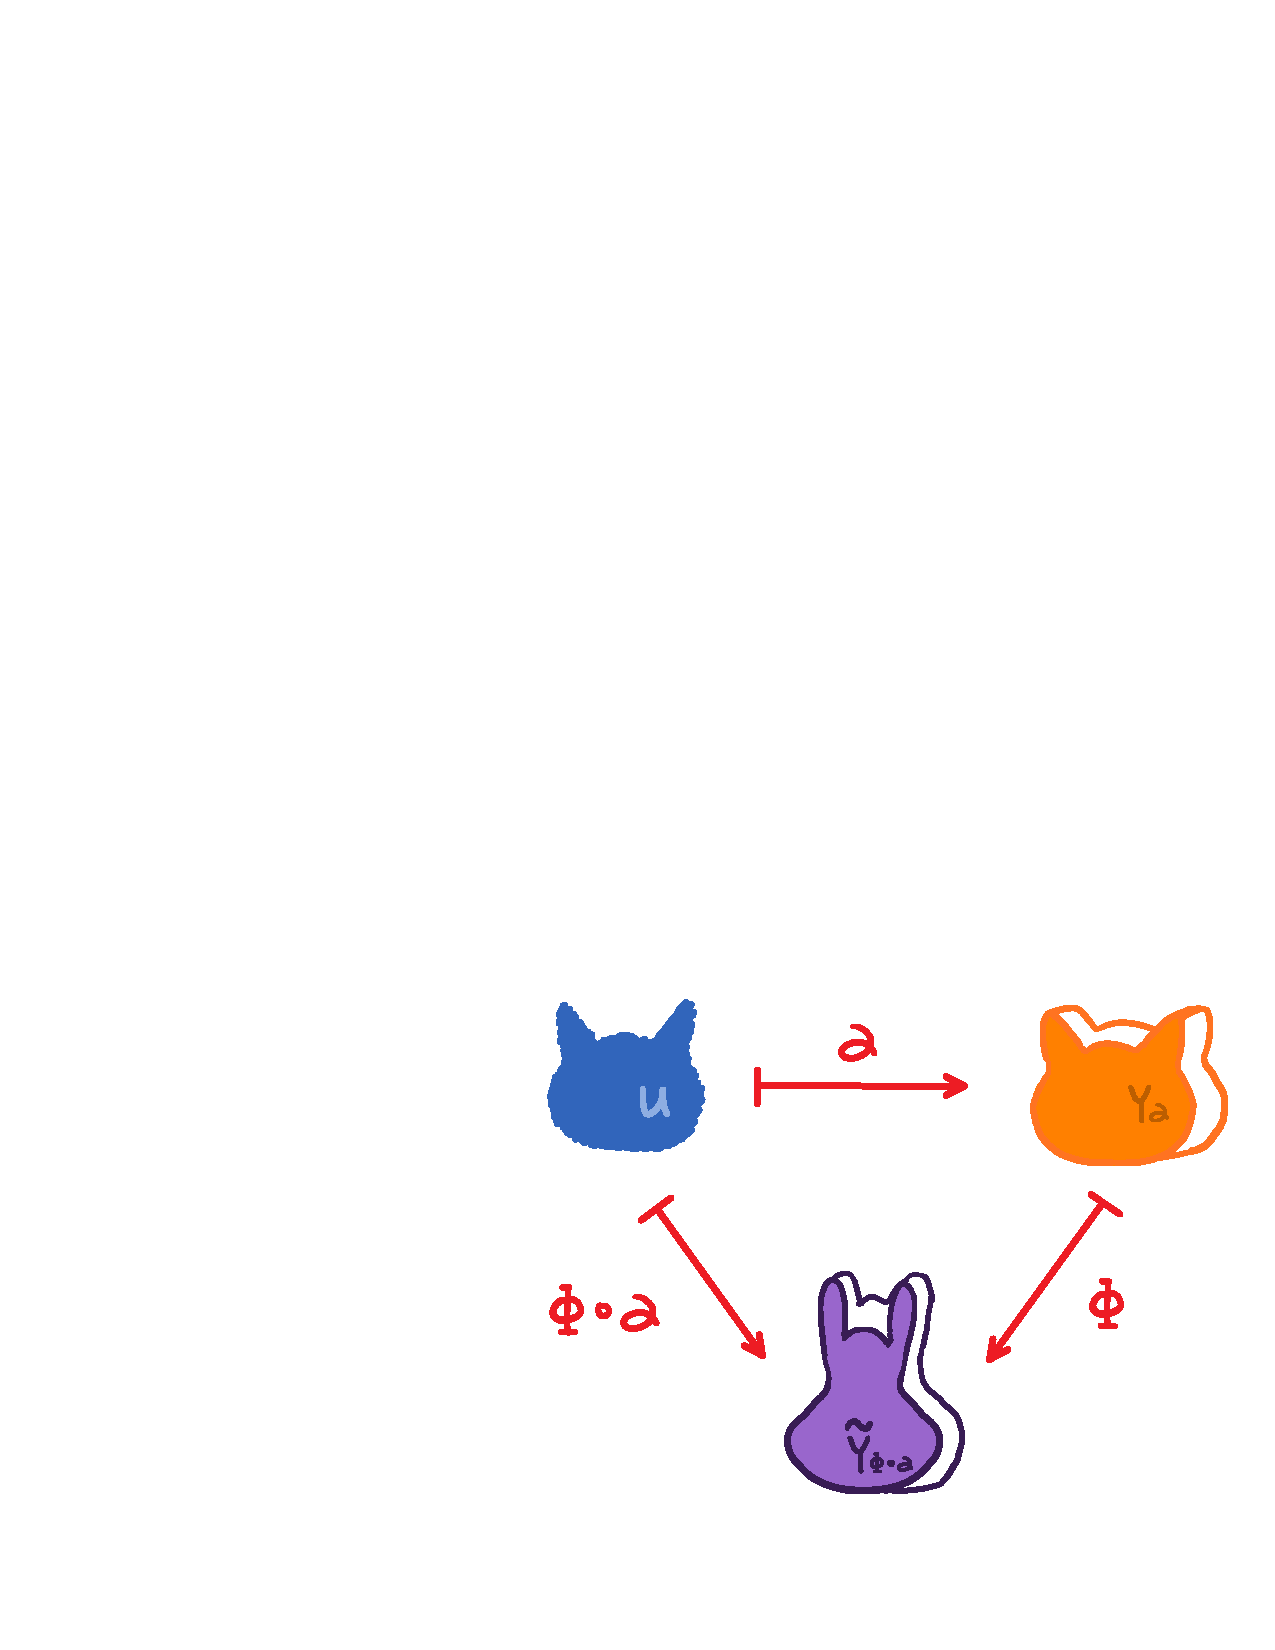
\includegraphics[scale=0.6]{Intkform1.pdf}\\
			\hfill\break
			\color{gray}Figure 0. Integrating k-form over a manifold\\is independent on the use of coordinate patches\color{black}
			
			
			
			\vspace{5cm}
			\LARGE
				\textbf{Jinyan Miao}\\
				\hfill\break
				\LARGE Fall 2022\\
			\vspace{1cm}

		\vspace*{\fill}
		\end{center}			
	\end{titlepage}


\newpage
\tableofcontents
\addtocontents{toc}{~\hfill\textbf{Page}\par}


\chapter*{Lab 9 - Square Well Simulation}
\section{Introduction}
\setcounter{chapter}{9}
In the theory of quantum mechanics, particles in a microscopic system, such as electrons orbiting a nucleus, or small particles confined in a quantum well, are described by the Schrodinger Equation:
\begin{align}
-\frac{\hbar^2}{2m}\nabla^2\psi + V\psi = i\hbar \frac{\pd}{\pd t}\psi
\end{align}
where $\psi$ is the wave function of the particle, $m$ is the mass of the particle, $V$ is the potential of the particle. Here $|\psi|^2$ gives the probabilistic distribution of the position of the particle in space. Solving the Schrodinger Equation under different boundary conditions gives rise to many interesting quantum phenomena. In Lab 9 of Physics 391, we investigate some of the many quantum phenomena predicted by the Schrodinger Equation. We simulate the situation where we have one or many finite quantum wells using a program developed by the University of Colorado. In the first part of the experiment, we investigate the behavior of quantum bound states in one or many quantum wells, we numerically verify the wavelengths of the Balmer series, and we verify that the number of bound-state solutions of the potential is approximately linear in the length $L$ of the quantum well. In the second part of the experiment, we investigate the scattering and tunneling effect in the quantum well and in the step potential. \\

\section{Experimental Setup}
The first part of the experiment is performed using the PhET \textit{Quantum Bound States} simulation program developed by the University of Colorado.\footnote{https://phet.colorado.edu/en/simulation/bound-states}\\

The second part of the experiment is performed using the PhET \textit{Quantum Tunneling and Wave Packets} simulation program developed by the University of Colorado.\footnote{https://phet.colorado.edu/en/simulation/quantum-tunneling}\\



\newpage
\section{Data Analysis}
\subsection*{Quantum Bound States}
\subsection{Coulomb Potential}
For the first part of the experiment, we first compute numerically the wavelengths of the Balmer series. We set the potential in equation (9.1) to be the Coulomb potential in $3$-dimensional space. The energy levels of the bound states and some statistics calculated from the numerical value of $E_n$ read the following:
\begin{center}
\begin{tabular}{|c|c|c|c|c|}
\hline
level $n$ & energy $E_n$ (eV) & $\lambda_n$ (nm)& $\lambda_{t,n}$ (nm) & name of line\\
\hline
1 & -13.7 & - & - & - \\
\hline
2 & -3.50 &- &- &-\\
\hline
3 & -1.61 & 656.00 & 656.27 & $\alpha$-line \\
\hline
4 & -0.95 & 486.21 & 486.13 & $\beta$-line \\
\hline
5 & -0.64 & 433.51 & 434.05 & $\gamma$-line  \\
\hline
6 & -0.48 & 410.54 & 410.17 & $\delta$-line \\
\hline
7 & -0.38  & 397.38 & 397.01 & $\epsilon$-line \\
\hline
8 & -0.31  & 388.66 & 388.91 & $\zeta$-line \\
\hline
9 & -0.27  & - & - &- \\
\hline
\end{tabular}
\end{center}
where $\lambda_n$ is calculated by the following:
\begin{align*}
\lambda_n = \frac{hc}{E_n-E_2}
\end{align*}
and $\lambda_{n,t}$ is the corresponding theoretical value for the wavelength of the emitted photon when the electron in a Hydrogen atom transits from $n$-th energy level to the second energy level, giving rise to the Balmer series. A simple observation here, we see that the numerical values of $\lambda_n$ that we calculate from our data are very close to the theoretical values $\lambda_{n,t}$. One should note that we are not able to confirm whether our data agree with the theoretical values because there is no error estimation for the energy levels in the simulation program. \\

\subsection{Single Finite Well}
Now we consider the case where we have finite square well potential $V_0 = 15\, eV$, and width of the well $L=1.5$. The energy levels are given by the followings:
\begin{center}
\begin{tabular}{|c|c|c|c|}
\hline
level $n$ & energy $E_n$ (eV) & characteristic time $\tau_n$ (fs)& number of nodes in $\psi$ \\
\hline
1 & 0.15 & 28.38 & 0\\
\hline
2 & 0.58 & 7.09 & 1\\
\hline
3 & 1.31 & 3.16 & 2\\
\hline
4 & 2.33 & - & 3\\
\hline
5 & 3.63 & - & 4\\
\hline
6 & 5.21 & - & 5\\
\hline
7 & 7.06 & - & 6\\
\hline
8 & 9.17 & - & 7\\
\hline
9 & 11.50 & - &8\\
\hline
10 & 13.97 & - & 9\\
\hline
\end{tabular}
\end{center}
where we measure the characteristic time of the wave function only for the first three energy levels, and in the following calculation, we see that they are very close to the values $\tau_{n,c}$ calculated by using the observed energy levels $E_n$:
\begin{align*}
\tau_{1,c} = \frac{h}{E_1} = 27.6\, fs \qquad\qquad
\tau_{2,c} = \frac{h}{E_2} = 7.13\, fs \qquad\qquad
\tau_{3,c} = \frac{h}{E_3} = 3.16\, fs \qquad\qquad
\end{align*}
There is no way we can do error calculation here because error estimations are not indicated in the simulation program. For simple observation, we see here that the wave functions for odd energy levels are even functions, and that for even energy levels are odd functions. The number of nodes in energy level $E_i$ is $i-1$. 
\begin{center}
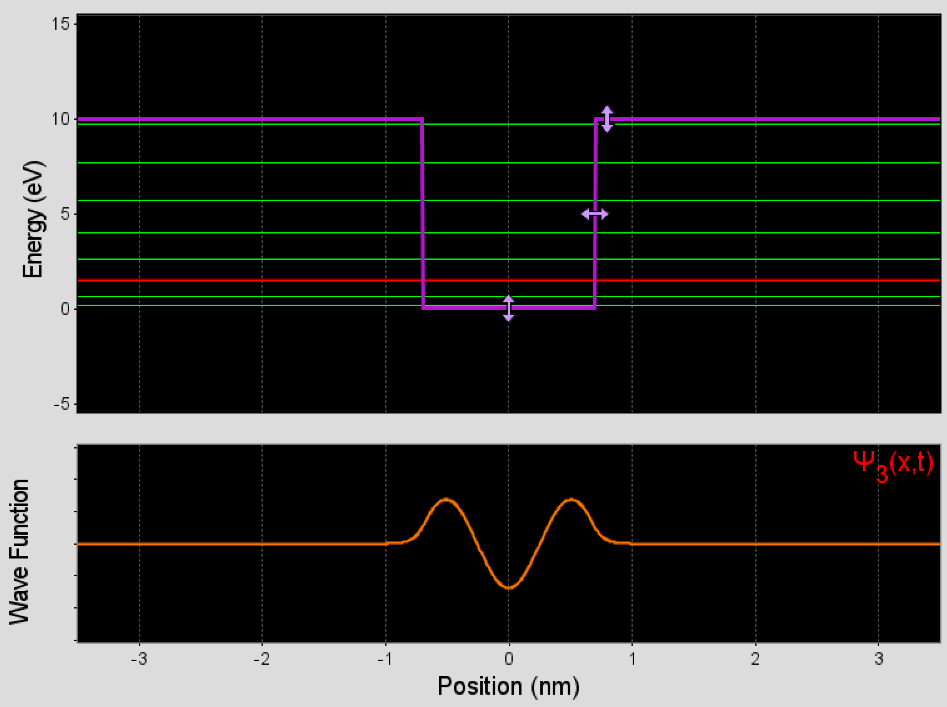
\includegraphics[scale=0.38]{1a}
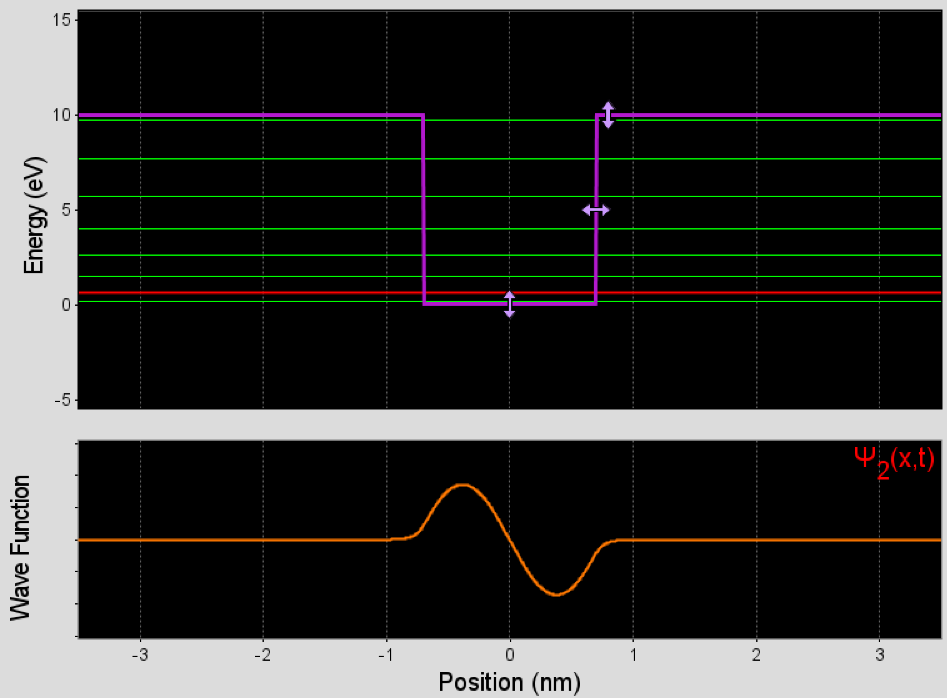
\includegraphics[scale=0.38]{1b}
\end{center}
\hfill\break

Here we plot the logarithm of the energy levels $E_n$ over the logarithm of the levels $n$ and perform a linear regression on the data points:
\begin{center}
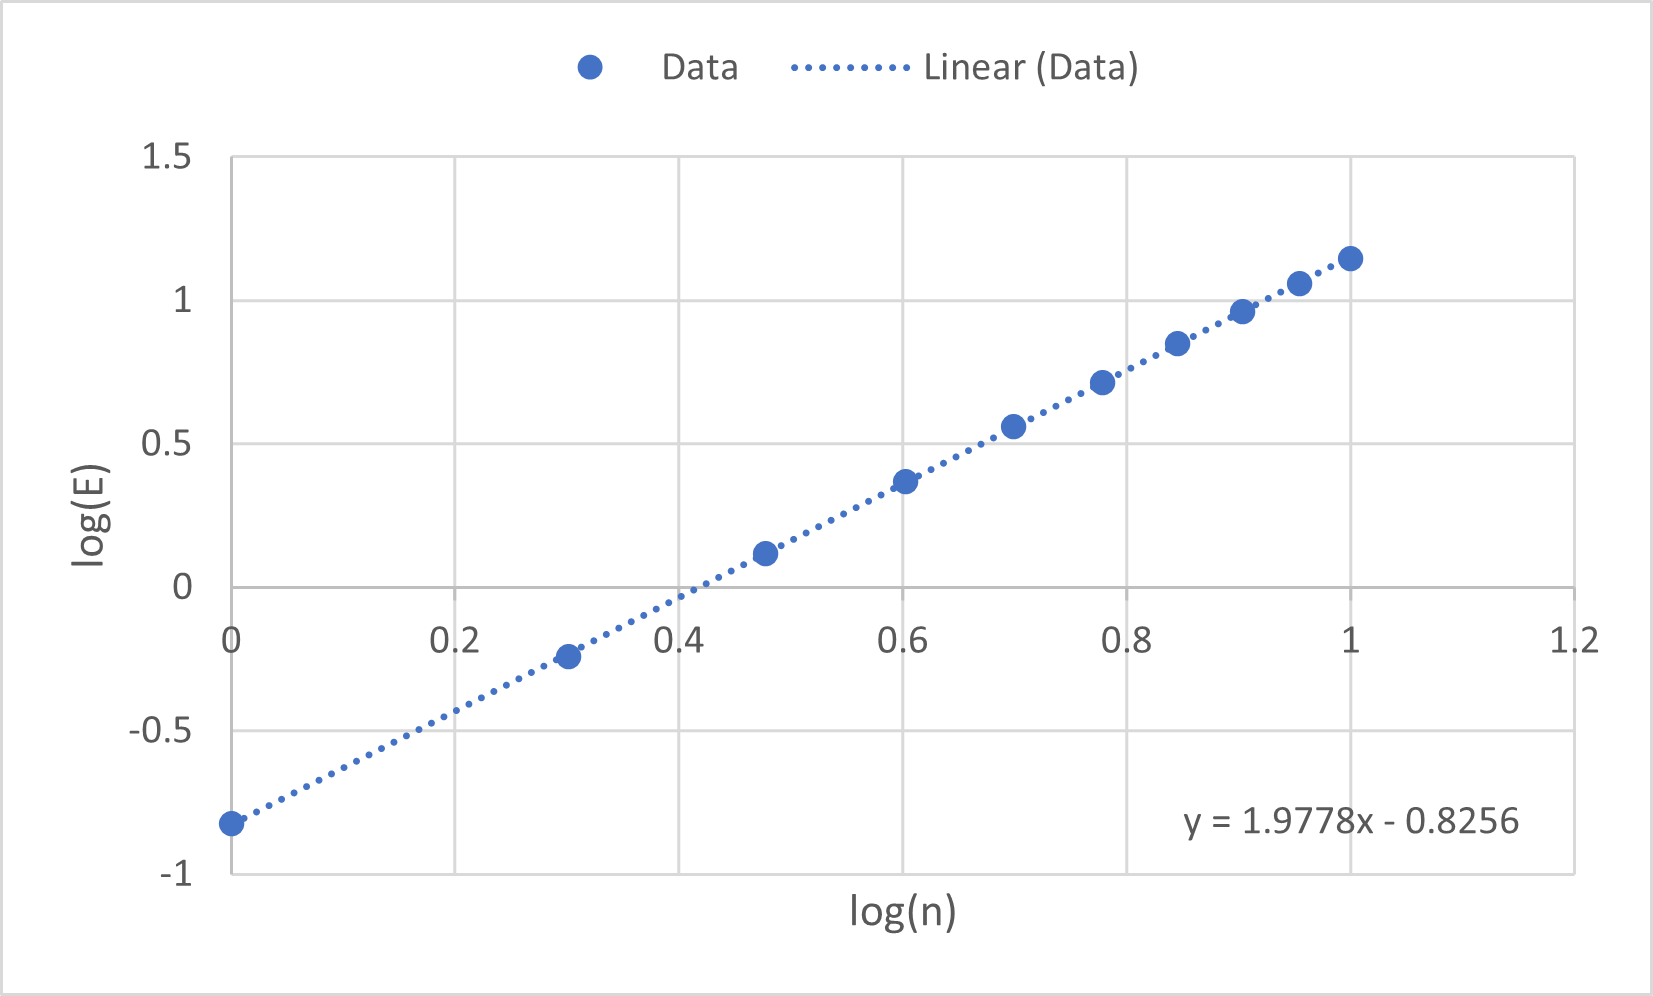
\includegraphics[scale=1.19]{1}
\end{center}
The slope of the regression line indicates the power dependence of $E_n$ on $n$. We observe that the indicated relation is approximately $E_n \propto n^2$. The standard deviation of the slope is given by $0.0043$, and the standard deviation of the $y$-interception is $0.0031$. This result makes sense because we have a dependence of $E_n \propto n^2$ in the case of an infinite square well:
\begin{align*}
E_n = n^2 \frac{\pi^2 \hbar^2}{2mL^2}
\end{align*}
One should expect a similar dependence behavior for the bound state energy levels in the case of a finite quantum well. Moreover, for three different lengths $L = 1.5,\ 3,\ 4.5$, in the unit of nm, we observe that the number of bound states in the finite square well system with fixed $V_0 = 15\, eV$ is given by $10$, $19$, $29$, respectively. Linear regression (without $y$-intercept) yields: 
$$n = (6.333\pm 0.192)\cdot 10^9 \, L$$ 
We note that the coefficient of $L$ is approximately given by:
\begin{align*}
\mathcal{C} = \frac{2\sqrt{2V_0  m_e} }{h} \approx 6.3155 \cdot 10^{9}
\end{align*}
we see here $\mathcal{C}$ is captured by our experiment value of $6.333$ within $1$-$\sigma$, hence the theoretical value of the coefficient in linear dependence of $n$ on $L$ is well predicted by our data. 
\begin{center}
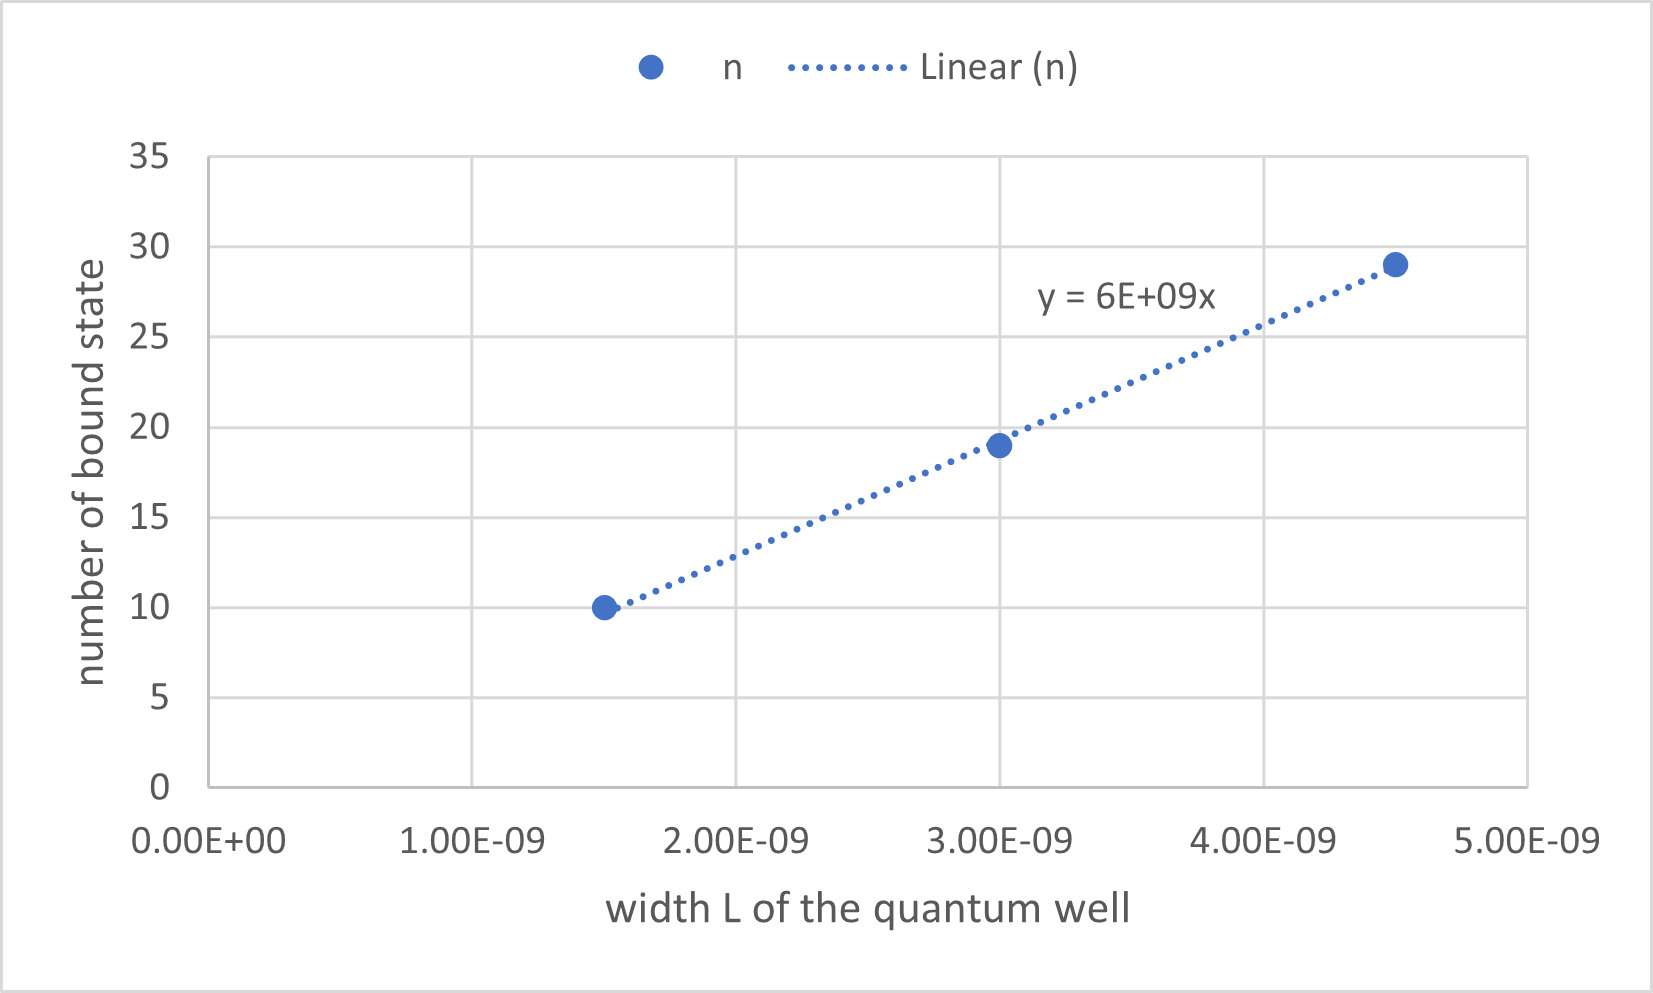
\includegraphics[scale=1.19]{2}
\end{center}

\subsection{Multiple Wells System}
In this section, we simulate a system consisting of many wells placed side by side, and investigate the behavior of the wave functions of the system. First, we perform the simulation for two wells of equal width and equal finite potential. Note that energy levels as seen in the single well system are now split into pairs with small energy gaps, here we call each pair a band. We observe that the upper energy level in a band has a wave function of odd symmetry (antisymmetric), and the lower energy level in a band has a wave function of even symmetry (symmetric). We also notice that, for each band, the upper-level wave function is obtained as if flipping either one side (with respect to the symmetry axis) of the lower-level wave function. When the separation of the wells increases from 0.1 nm to 0.7 nm, the upper and the lower energy levels in a band degenerate to a single energy level, and the wave function for each energy level is equivalently the sum of the two single-electron wave functions confined in two separate wells.
\begin{center}
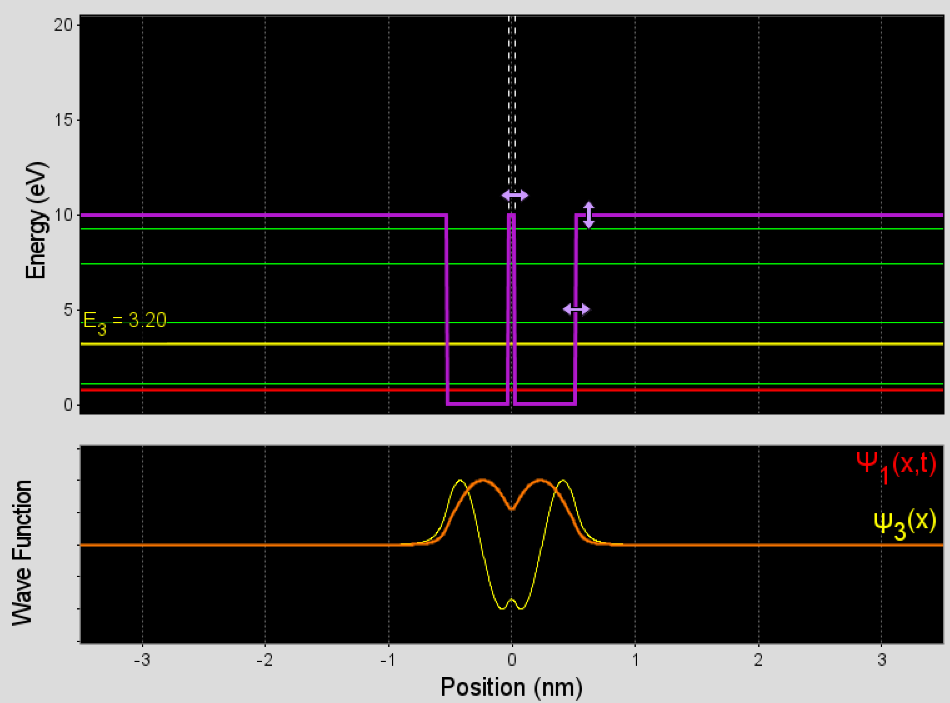
\includegraphics[scale=0.38]{2a}
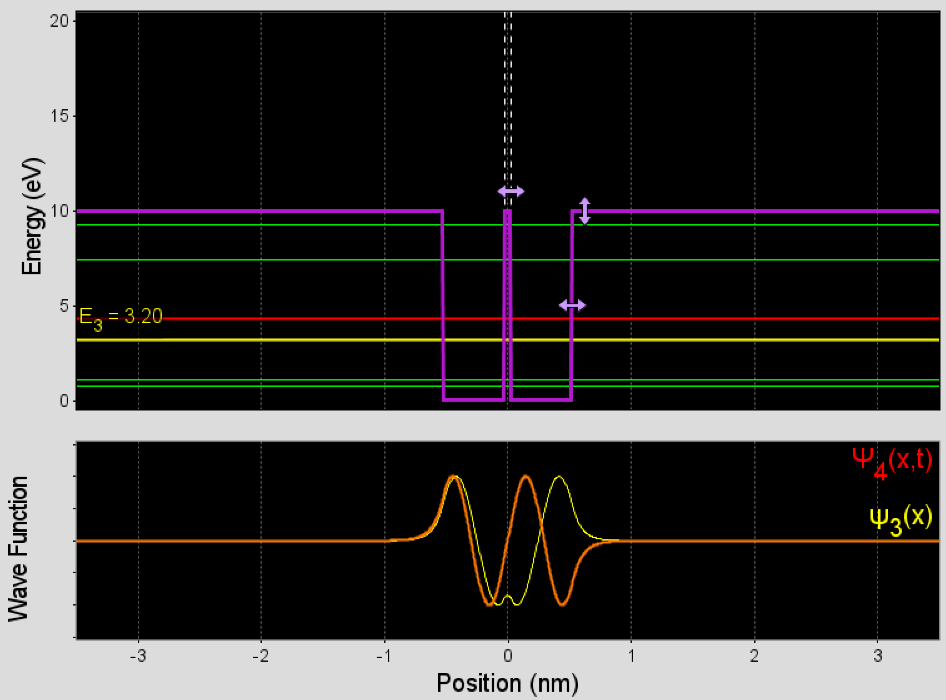
\includegraphics[scale=0.38]{2b}\\
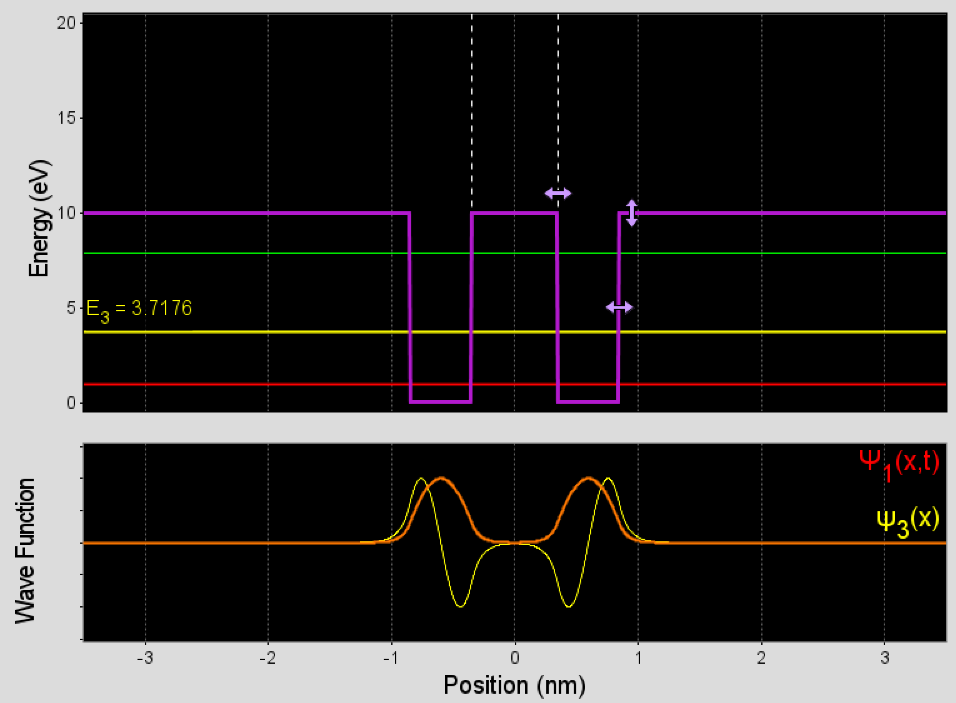
\includegraphics[scale=0.38]{2c}
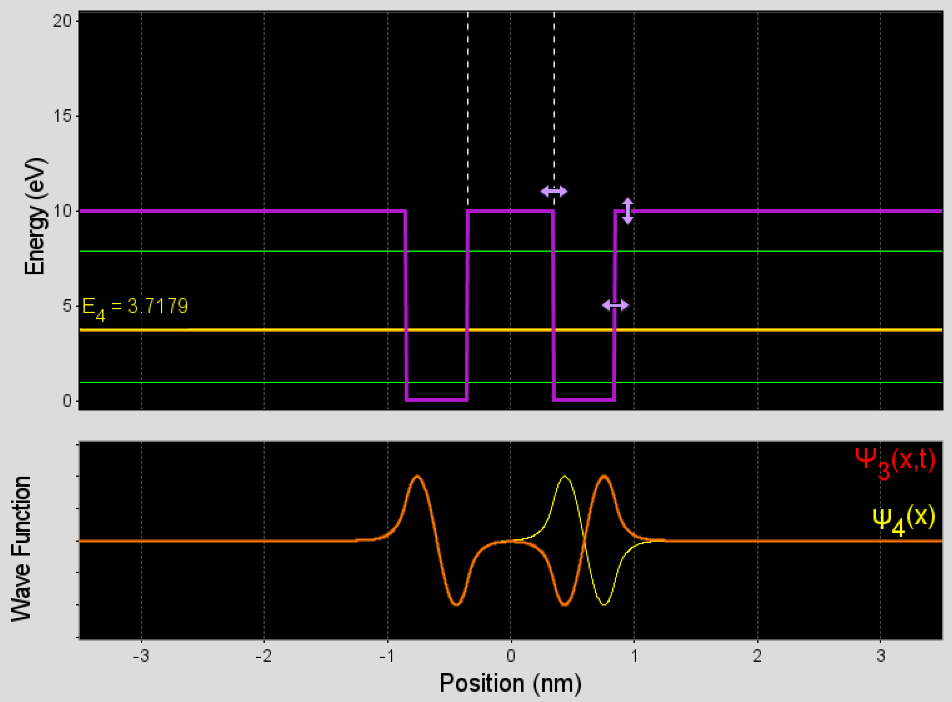
\includegraphics[scale=0.38]{2d}
\end{center}

We can think of the two-well configuration as the molecular bounding in a diatomic hydrogen molecule, where the two protons in the system serve as two finite wells, or the two potentials that confine an electron. An electron in such a two-well system can travel in such space and its position is characterized by its wavefunctions. There is a nonzero probability that the electron can tunnel from one of the wells to the other, but such a probability is small enough to be neglected when the wells are separated far away. The wavefunctions of the single electron can be symmetric and antisymmetric. When the two wells are far apart, the energies of each pair of symmetric-antisymmetric wavefunctions degenerate, but when the wells are brought near together, the degeneracy is lifted, hence resulting in the split of energy levels of the electron. The antisymmetric wavefunction in this case has energy higher than the symmetric one. \\

Now we put more wells into the system, say, 10 wells. We observe that there are 10 energy levels in each band, and the pattern still follows that odd levels have even wavefunctions, and even levels have odd wavefunctions.
\begin{center}
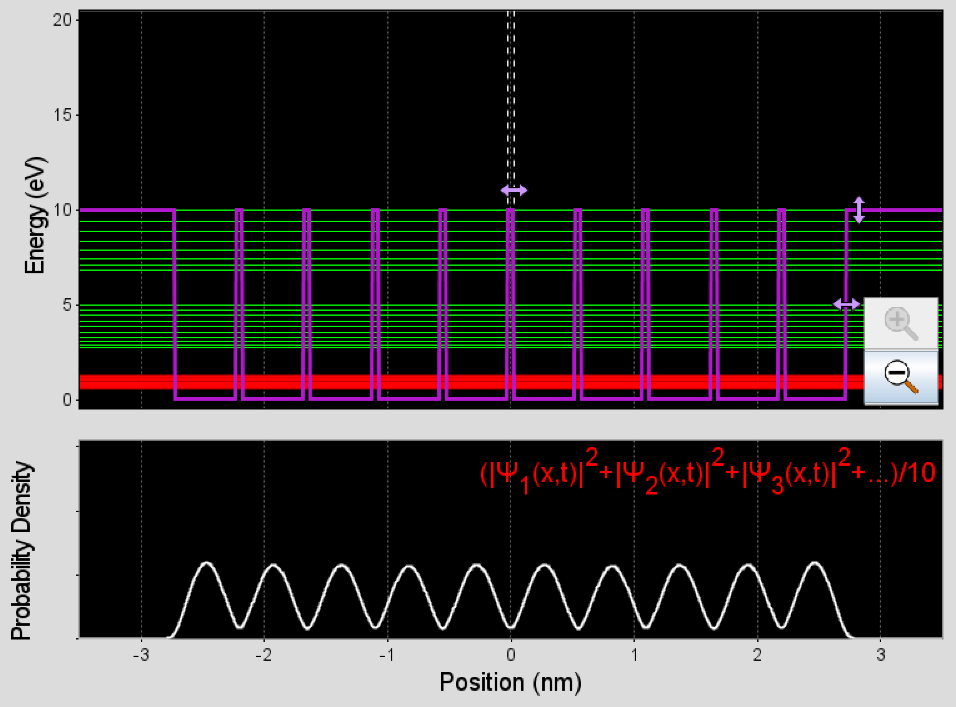
\includegraphics[scale=0.38]{3a}
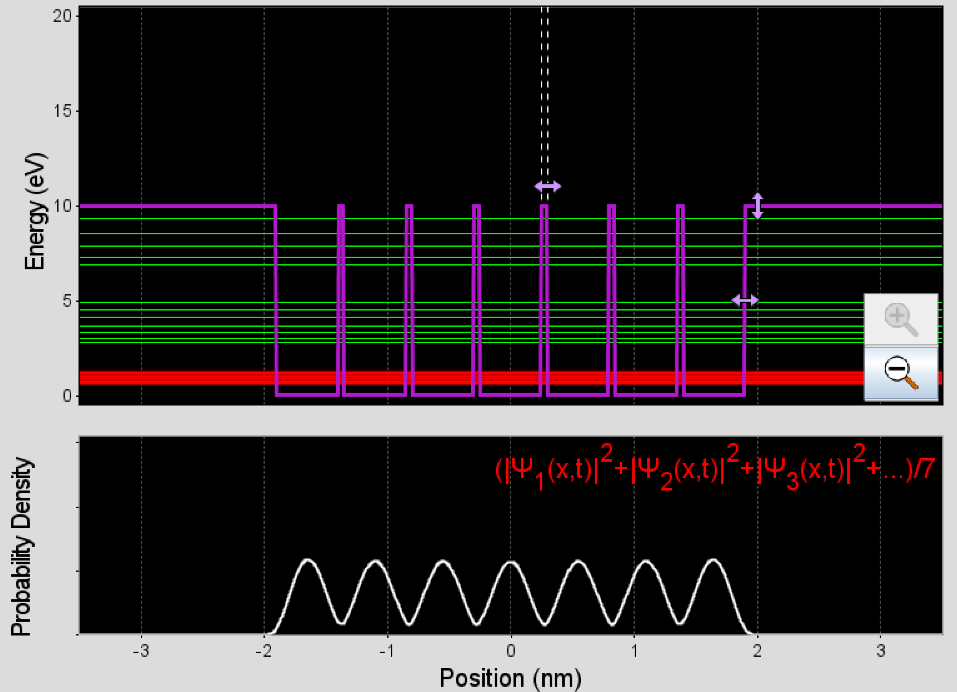
\includegraphics[scale=0.38]{3b}
\end{center}
For the probability density function of a band that has a higher energy level, the horizontal span in space is approximately the same as that of the lower energy level, but the number of regional maxima in the density function is more than that of the lower energy level. When the spacing between the wells increases, we see again that the energy levels in each band tend to degenerate into a single energy level. Moreover, the change in the number of wells does not have a significant effect on the width of the band, assuming that the spacing, width, and height of the wells are unchanged. \\

\subsection*{Scattering and Tunneling}
\subsection{Step Potential}
In the following discussion, if not specified, we assume that the incoming wave goes from the left to the right. For a step potential $0\to V_0$. If the total energy $E$ of the propagating wave is greater than $V_0$, we see that the wave can propagate through the step potential and result in a sinusoidal wave on the right-hand side of the step. The transmission coefficient $T$ of the wave is relatively large and nonzero. On the left-hand side of the step, the reflected coefficient $R$ is relatively small but nonzero, and hence the incoming wave on the left of the step superimposes with the reflected wave, forming an amplitude-oscillating sinusoidal wave propagating to the right. If we flip the step to $V_0 \to 0$, $T$ and $R$ remain unchanged. In the case where we have the step $0\to V_0$, if we have $E<V_0$, we see that the wave on the left-hand side of the step is an amplitude-oscillating sinusoidal standing wave, while on the right-hand side of the step, the wave attenuates exponentially. The transmission coefficient in this case is zero, and the reflected coefficient is $1$. Denote the potential on the left of the step as $V_1$, the potential on the right of the step as $V_2$, and the total energy of the particle as $E$.\\

Here we plot $T$ and $R$ as functions $V_1$, keeping $V_2=0\, eV$ and $E=0.5\, eV$:
\begin{center}
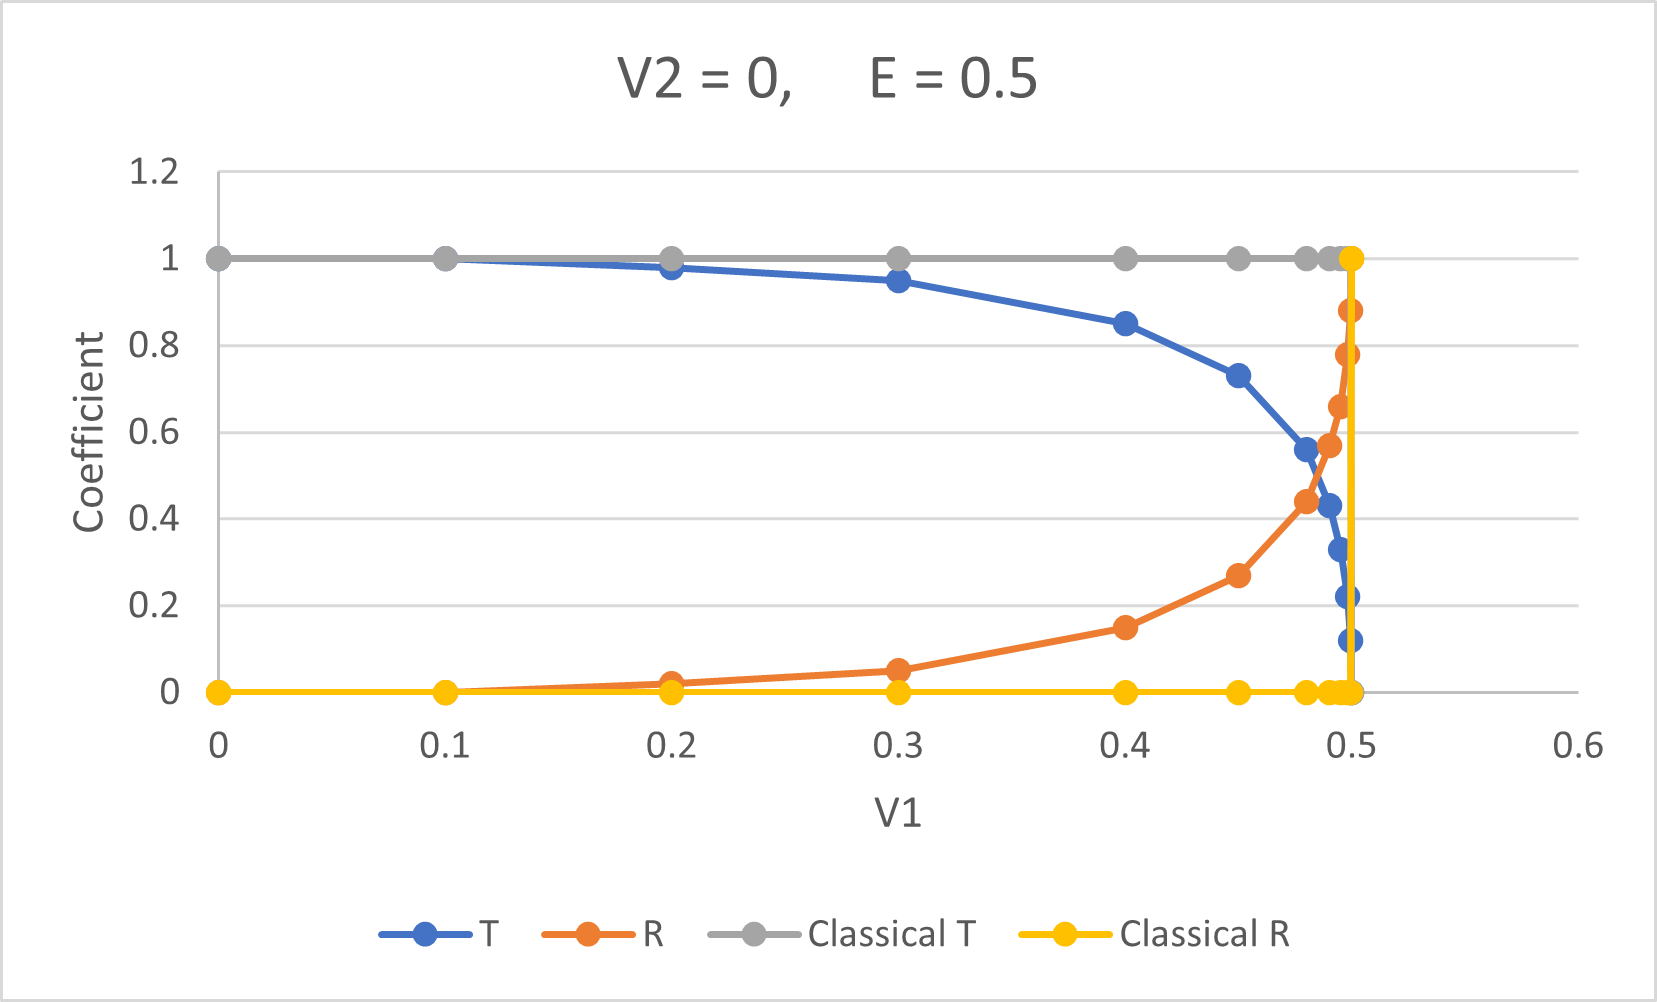
\includegraphics[scale=1.19]{TR1}
\end{center}
Notice that when $V_1 >E$, no particle exists on the left of the step. Classically, whenever we have $V_1 < E$,$T=1$ and $R=0$, hence there is a jump at $V_1 = E$ in the classical theory. But in quantum mechanics, we see here $R\neq 0$ and $T\neq 1$ even for $V_1<E$. \\

Now we plot $T$ and $R$ as functions $V_2$, keeping $V_1=0\, eV$ and $E=0.5\, eV$:
\begin{center}
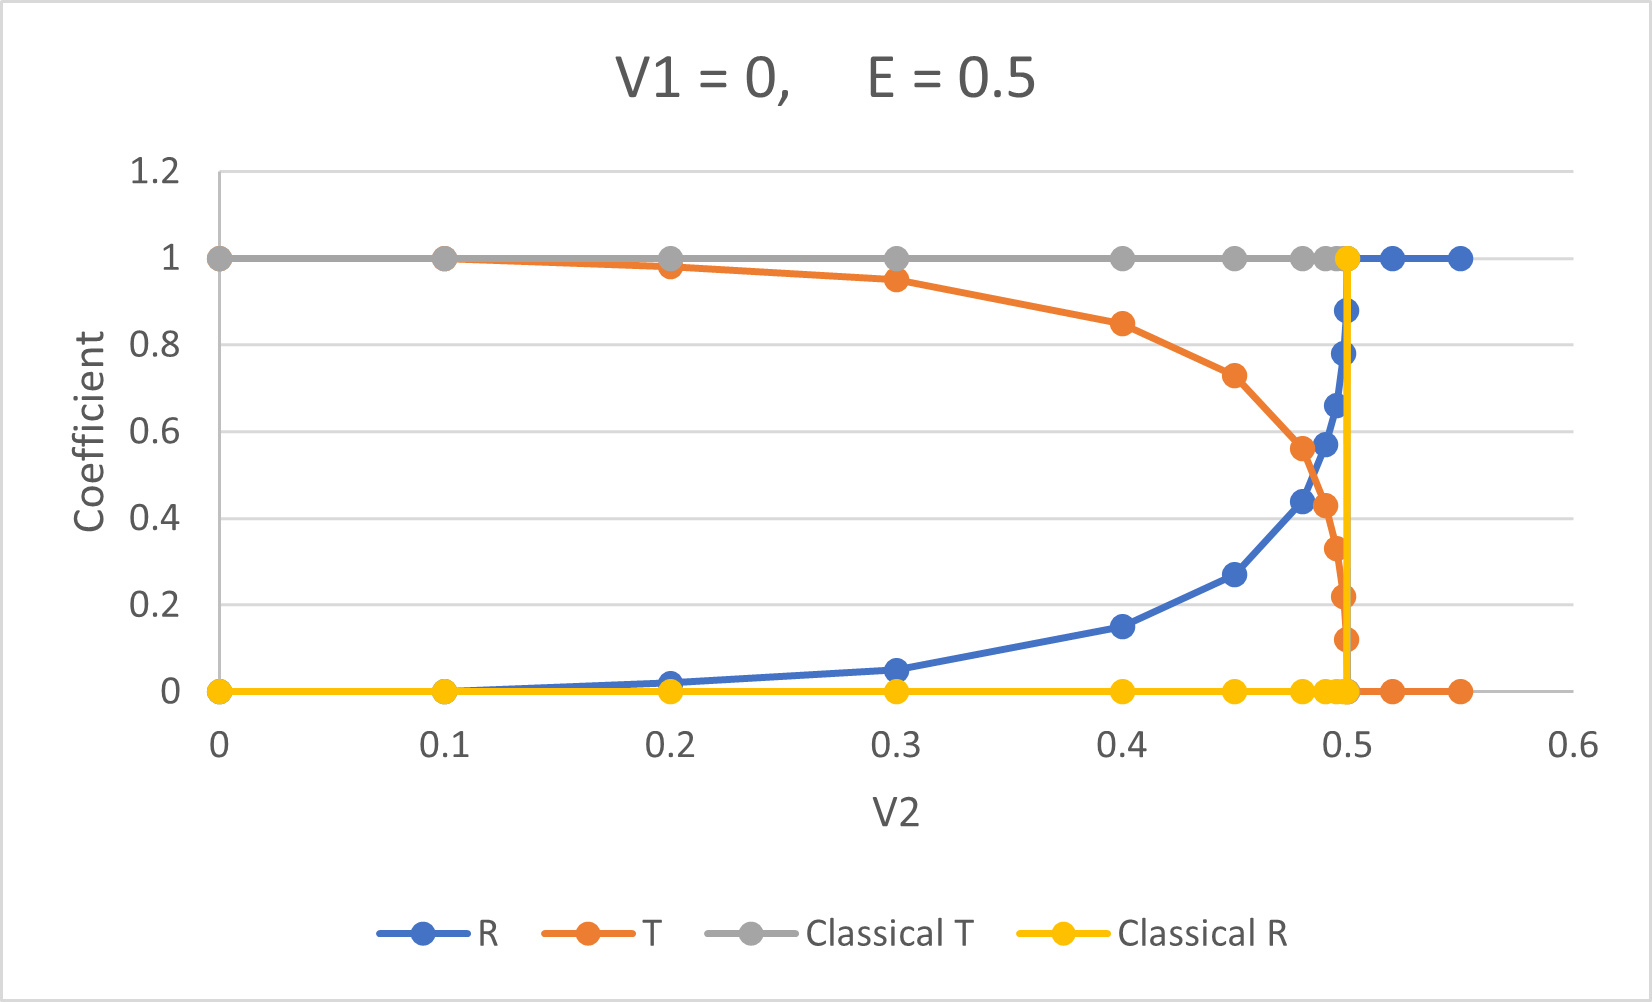
\includegraphics[scale=1.19]{TR2}
\end{center}
In this configuration, we are allowed to have $V_2>E$, in which case $T=0$ and $R=1$ for both classical and quantum theory. We expect to see a jump at $V_2 = E$ from classical theory, but in quantum theory $R\neq 0$ and $T\neq 1$ even in the region $V_2<E$.\\

\subsection{Square Barrier}
Now we set up the simulation where we have an incoming wave going from the left to the right. There is a square potential barrier of width $1\, nm $ and height $V_2=0.5\, eV$ in the middle. On the left and right of the barrier, we have potential $V_1 = V_3 = 0\, eV$. The incoming wave has total energy $E=0.5\, eV$. In this situation, $T$ and $R$ are plotted below:
\begin{center}
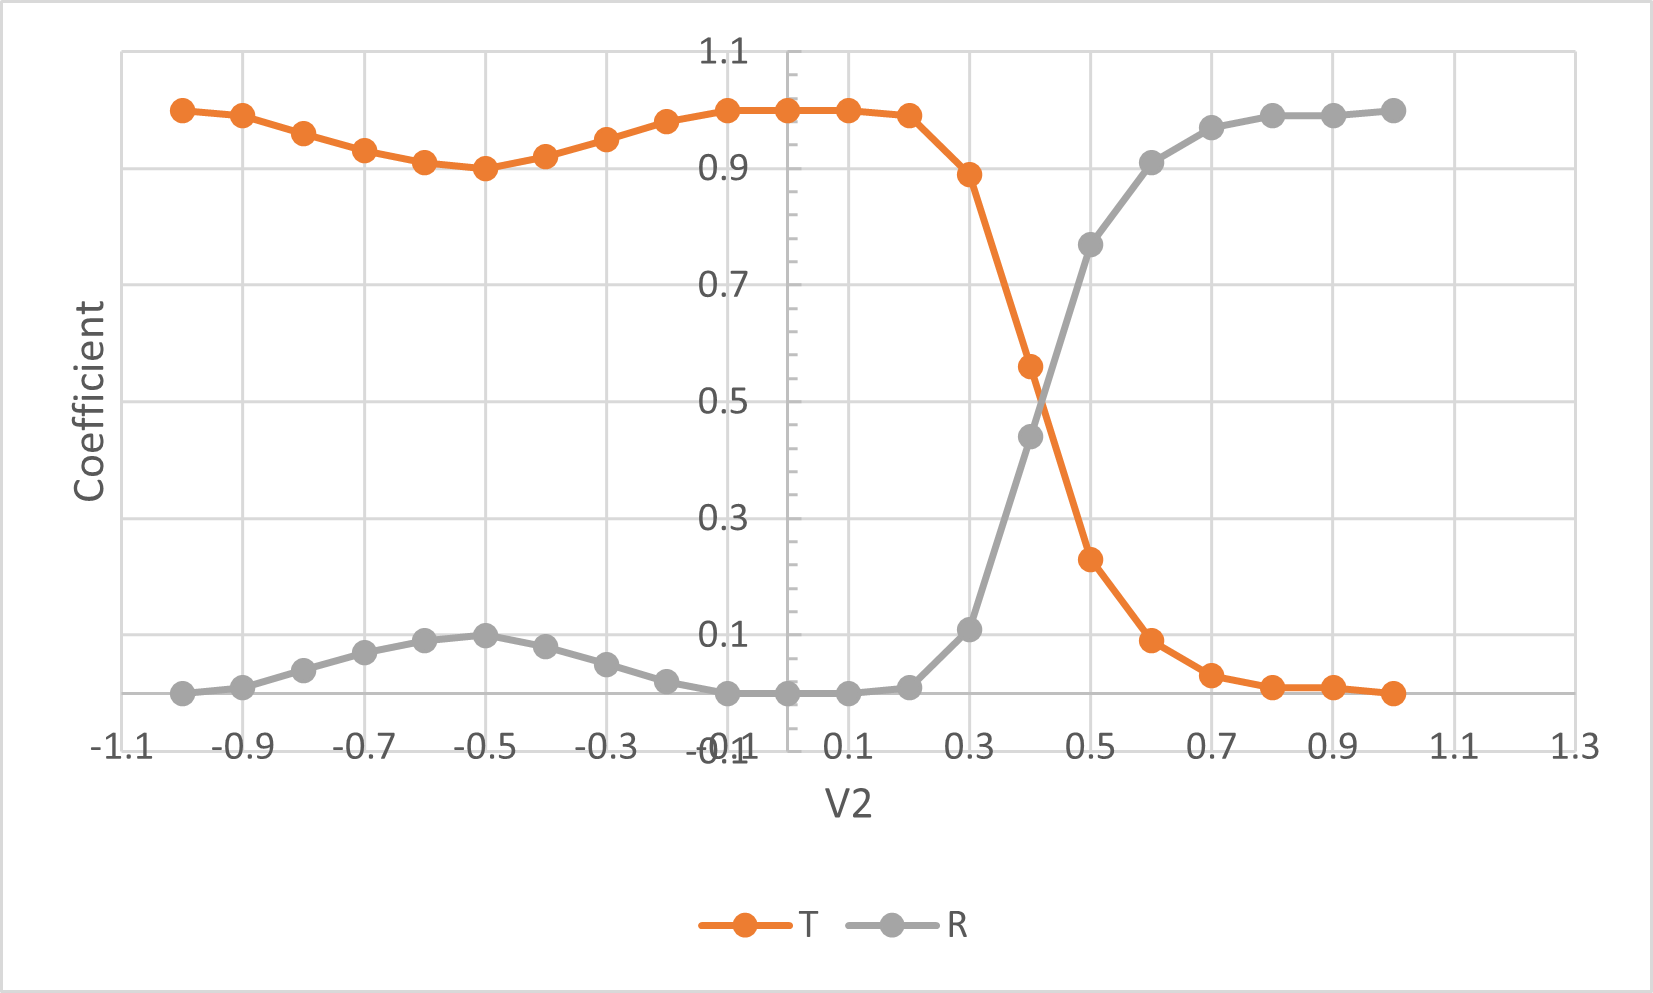
\includegraphics[scale=1.19]{Tunnel}
\end{center}
where we see here there is a rapid increase in $T$, and a rapid decrease in $R$, at around $V_2 = E = 0.5\, eV$. In classical theory, we expect $T=0$ for $V_2 \geq E$, but this is not the case in quantum theory. The simulation result indicates that $T$ does not vanish in the region $V_2 \geq E = 0.5$, hence the particle has a probability of tunneling through the barrier and reaching the region $V_3$, even though the total energy of the particle might be smaller than the potential of the barrier $V_2$. We also see here $R$ is nonzero when $V_2 < E$, in contrary to the classical theory.\\

\subsection{Double Square Barrier}
In this section, we make a double barrier with $V_1 = V_3 = V_5 = 0$ and $V_2 = V_4 = 0.5 eV$.  The incoming particle goes through the system under the potential $V_1\to V_2 \to V_3\to V_4\to V_5$. The widths of the barriers are both $0.5\, nm$, and the quantum well formed by the two barriers has a width of $1.5\, nm$. The transmission and reflected coefficients are plotted as functions of the total energy of the particle $E$:
\begin{center}
\includegraphics[scale=1.19]{DoubleBar}
\end{center}
Here we see that there is a peak in the transmission coefficient at $E \approx 0.33$, and another peak at $E \approx 0.73$. The case at $E\approx 0.33 < V_2$ is of particular interest. In this case, the total energy of the particle is less than that of the barrier, but we have a transmission coefficient being $1$. It turns out that, the double barrier is totally transparent for particle transmission. This phenomenon is called resonant tunneling.

\subsection{Quantum Measurement}
Here we set the potential $V_0$ to be a constant, and the total energy of the traveling particle (from left to right) to be $E>V_0$. As time evolves, we see here that the wave function of the particle, and the corresponding probability density, spread out in space, while with a net speed traveling to the right. Here the net speed of the wavefunction refers to the speed of the wave packet of the particle. When we make a quantum measurement, the probability density and the wave function collapse at a well-localized region (with position predicted by the probability density function), and then diffuse again after the quantum measurement. For higher energy $E$, the particle travels faster, that is, the net speed of the wavefunction is greater for higher $E$. 




\section{Summary}
In Lab 9 of Physics 391, we used to PhET simulation program to investigate the behavior of wavefunctions of different bound states of an electron confined in one or many quantum wells, we numerically verify the wavelengths of the Balmer series. We also verify that the number of bound-state solutions of the potential is approximately linear in the length $L$ of the quantum well and determined to linear dependency coefficient. In the second part of the experiment, we investigated the scattering and tunneling effect in quantum well, and in step potential, we found the situation where the resonant tunneling occurs, and we observed the effect of making a quantum measurement. \\


\end{document}